% !TeX root = ../tango.tex
\section{TANGO Methodology}
\label{sec:tango-methodology}

Fig.~\ref{fig:tango-overview} shows the design overview of \tango{}, which comprises a \dispatcher{} and a \allocator{}.
At each iteration boundary, the two components coordinate request execution priority and per-step token allocation according to heterogeneous TTFT and TPOT SLOs.
They take each request's SLOs, inference phase, and execution progress as input and produce a mixed batch of prefill chunks and decode tokens.

\begin{figure}[t]
  \centering
  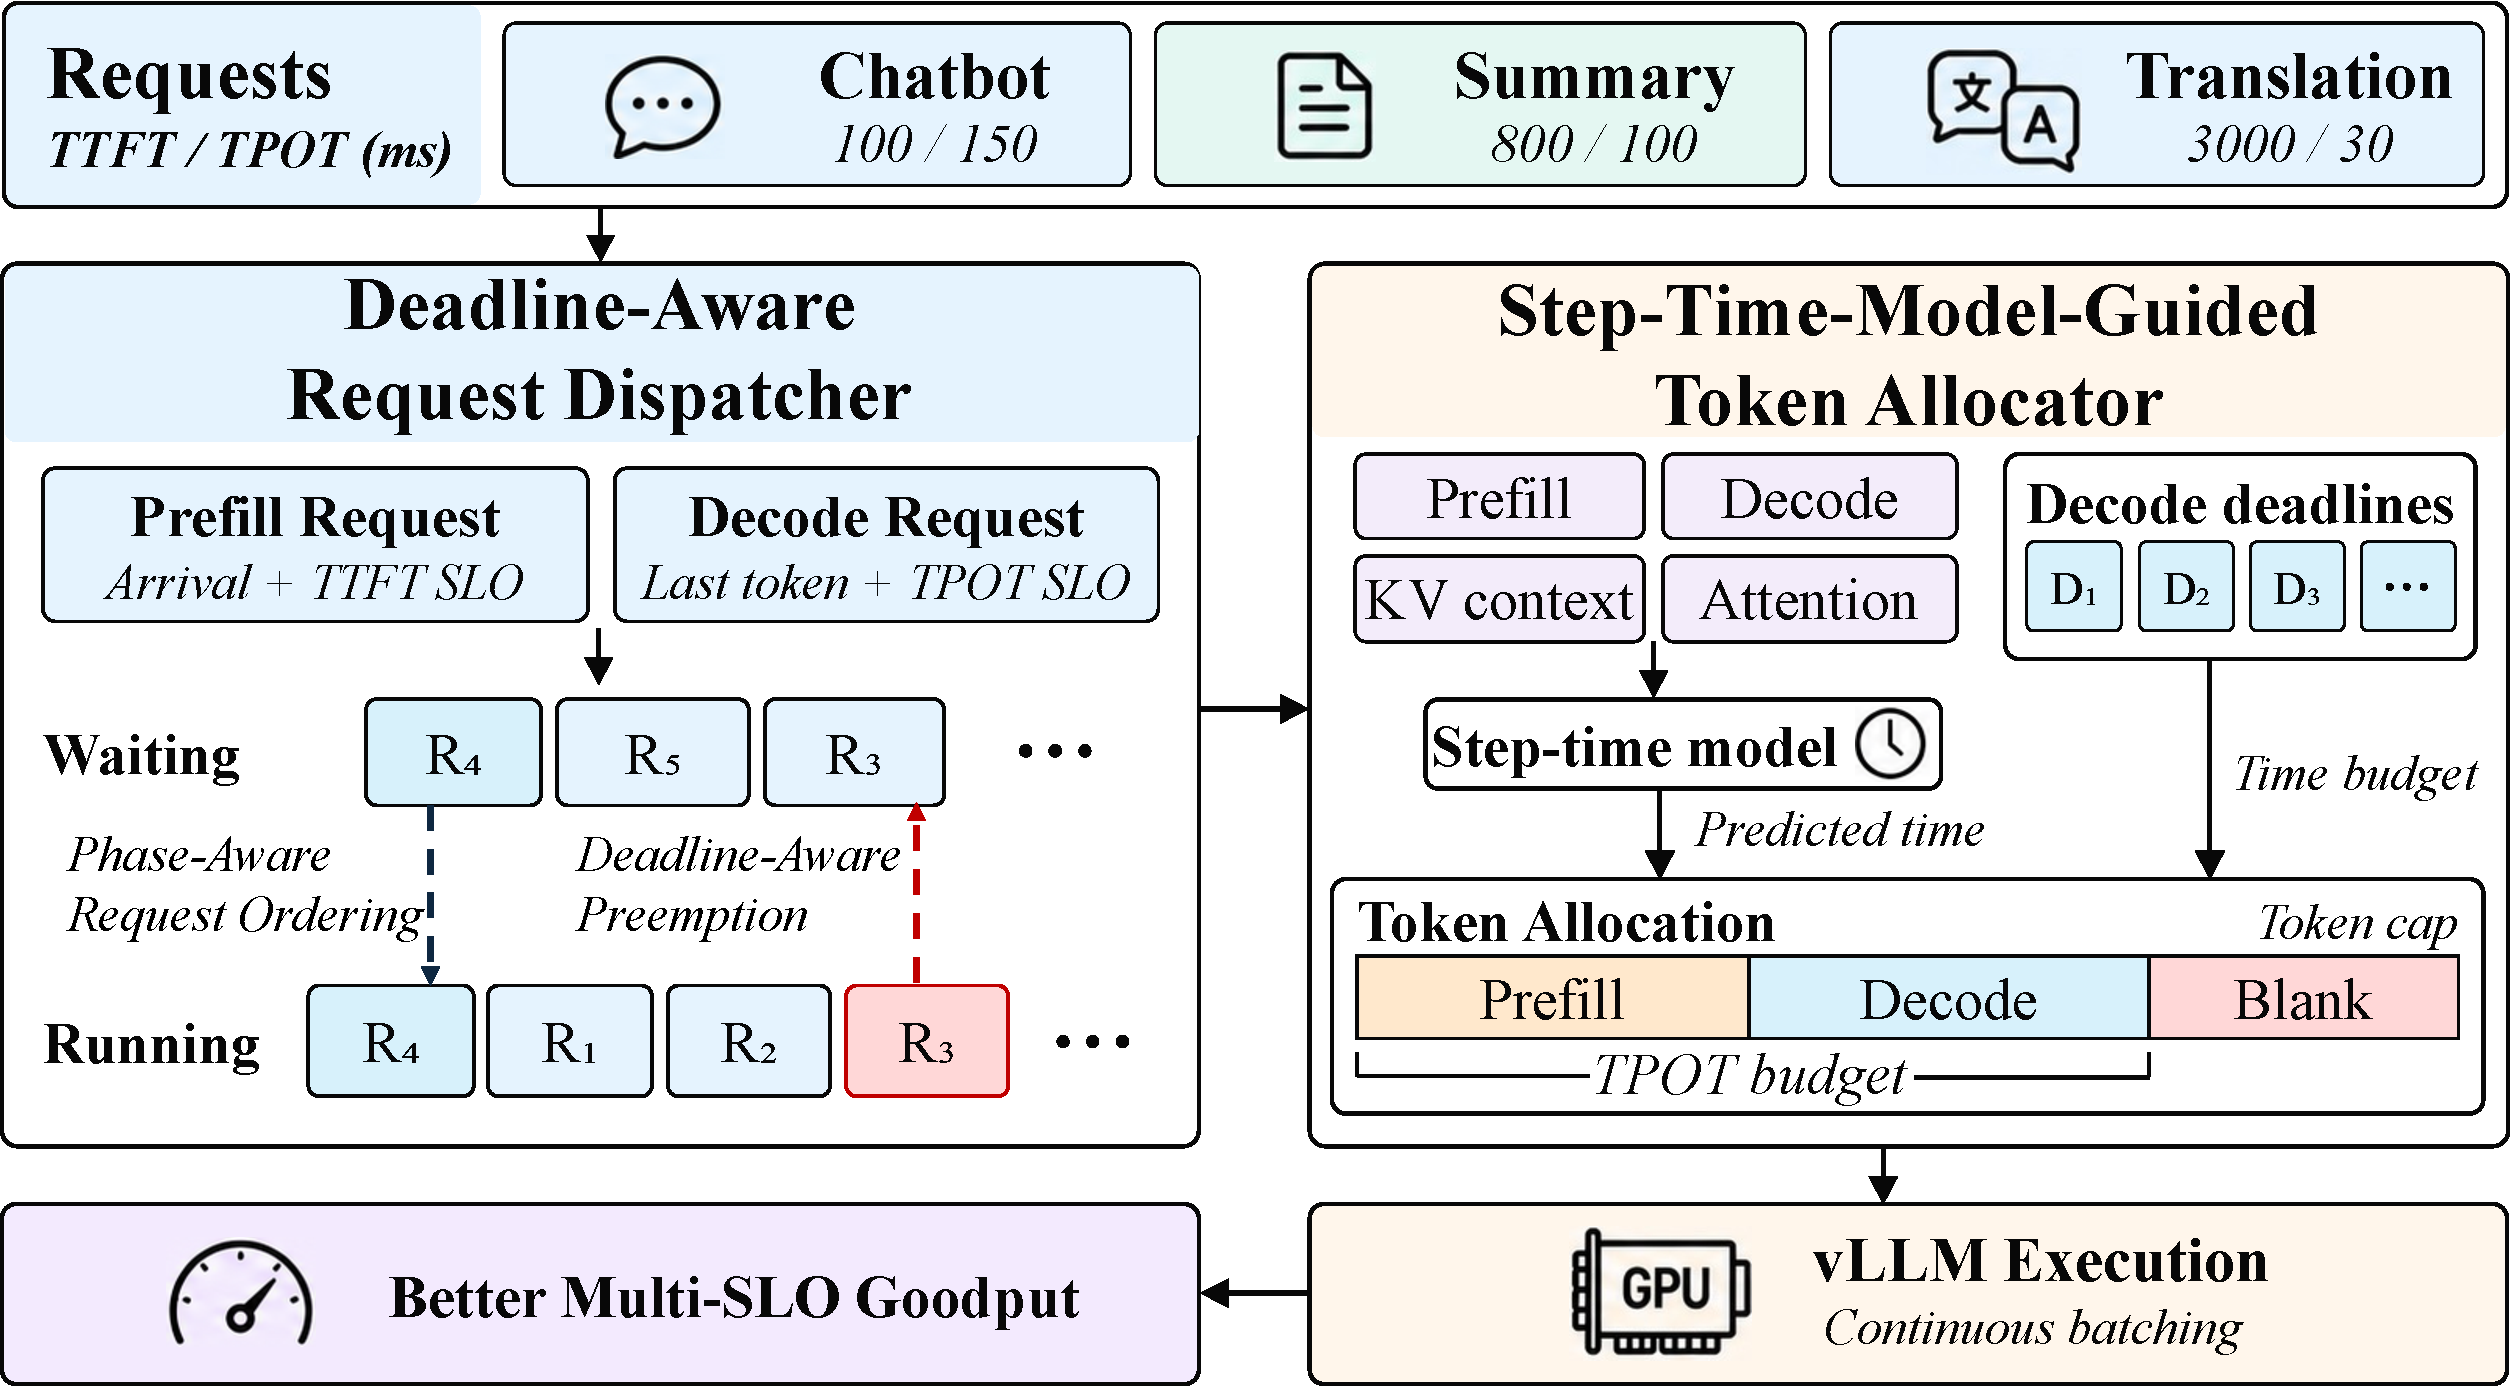
\includegraphics[width=\columnwidth]{figures/tango-methodology/overview}
  \caption{Design overview of \tango{}.}
  \label{fig:tango-overview}
\end{figure}

The temporal scheduling challenge is to compare request urgency across inference phases.
A request with an unfinished prefill must produce its first token within its TTFT budget, whereas a decoding request must sustain token-generation progress within its TPOT budget.
The dispatcher maps these phase-specific requirements to comparable deadlines and updates request priorities as inference progresses.
These priorities guide the admission of waiting requests and the preemption of less urgent ongoing requests under resource contention (Section~\ref{sec:deadline-aware-request-dispatcher}).

The spatial scheduling challenge is to advance urgent prefills while limiting their interference with decoding requests.
As shown in Section~\ref{subsec:motivation-underlying-reasons}, the total token count alone cannot reliably determine mixed-step execution time.
The allocator therefore uses a step-time model to predict the duration of candidate batches from their prefill/decode composition and context-dependent attention work.
It converts the remaining deadline slack of selected decode requests into a prefill token budget and distributes that budget according to the dispatcher's priorities (Section~\ref{sec:step-time-model-guided-token-allocator}).

Specifically, \tango{} operates as follows.
First, the scheduler collects the running requests' execution state, and the allocator derives a prefill token budget using the step-time model.
Second, the dispatcher orders waiting requests by their phase-aware deadlines for admission alongside ongoing requests.
If a waiting request cannot obtain KV-cache blocks, the dispatcher considers preempting the running request with the latest deadline, but proceeds only when the waiting request has an earlier deadline.
The allocator applies the remaining token and time budgets to the prefill chunks of ongoing and newly admitted requests.
Finally, the engine executes the resulting batch and returns token timestamps and request progress to update the next scheduling decision.
Unfinished requests remain eligible for reconsideration at the next iteration boundary.

The example in Fig.~\ref{fig:tango-overview} illustrates how the two components cooperate.
An urgent waiting request $r_4$ receives earlier admission, while a less urgent ongoing request can be preempted to release capacity.
The allocator then determines how much of the admitted request's prompt can share a step with the active decode workload.
When the decode requests have little remaining deadline slack, it limits the prefill chunk size and leaves the remaining prompt tokens for subsequent steps, even if the engine's maximum token capacity has not been exhausted.
Thus, request urgency determines the service order, while predicted step time determines how much work can execute in that order.

% !TeX root = ../tango.tex
\subsection{\dispatcher{}}
\label{sec:deadline-aware-request-dispatcher}

% TODO: Write this section.

% !TeX root = ../tango.tex
\subsection{\allocator{}}
\label{sec:step-time-model-guided-token-allocator}

% 第1段：结合执行流程图介绍 allocator 如何用预测步耗时将 decode 时间预算转为 prefill 配额；交代模型、联合预算和执行流程的结构。
Fig.~\ref{fig:token-allocator-workflow} shows how the allocator determines the amount of prefill work that can share an engine step with the active decode workload.
Its key idea is to translate the remaining next-token time budget into a prefill token allocation using a fitted step-time model.
In this section, we first introduce the model, then explain how heterogeneous TTFT and TPOT objectives guide budgeting, and finally describe the allocation workflow.

% 图注：简述 allocator 执行流程；虚线含义与符号说明见正文。
\begin{figure}[t]
  \centering
  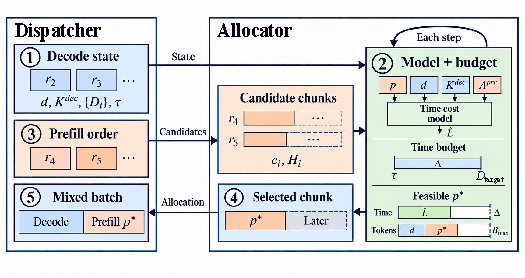
\includegraphics[width=\columnwidth]{figures/tango-methodology/token-allocator-workflow.pdf}
  \caption{Execution workflow of the \allocator{}.}
  \label{fig:token-allocator-workflow}
\end{figure}

\subsubsection{Step-Time Modeling}
\label{subsec:step-time-modeling}

% 第2段提纲：从固定 token 总数不能约束混合步延迟的问题出发，定义四个工作量特征并给出模型；沿用已有 p/d 及 batch 记号，避免与 request deadline D_i 混淆。
As analyzed in Section~\ref{subsec:motivation-underlying-reasons}, batches with the same total token count can have substantially different execution times.
The predictor must therefore account for both batch composition and context-dependent attention work.
Let $p$ and $d$ denote the numbers of prefill and decode tokens, respectively, $K^{\mathrm{dec}}$ the sum of context lengths accessed by decode requests, and $A^{\mathrm{pre}}$ the effective attention work of prefill chunks.
These four inputs feed the time cost model in Fig.~\ref{fig:token-allocator-workflow}, which estimates the step duration as
\begin{equation}
  \widehat{L}\!\left(p,d,K^{\mathrm{dec}},A^{\mathrm{pre}}\right)
  = \alpha + \beta p + \gamma d
    + \delta K^{\mathrm{dec}} + \epsilon A^{\mathrm{pre}}.
  \label{eq:step-time-model}
\end{equation}

% 第3段提纲：逐项解释模型与主要执行成本的对应关系，说明这些项是拟合得到的近似，而非每种操作的精确计时。
Each term approximates a different source of execution cost.
The intercept $\alpha$ captures the fixed runtime cost of a step, while $\beta p$ and $\gamma d$ capture the token-dependent costs of prefill and decode computation.
The term $\delta K^{\mathrm{dec}}$ accounts for decode attention's KV-cache reads, which grow with the total history accessed by decode tokens.
Finally, $\epsilon A^{\mathrm{pre}}$ accounts for the attention computation performed by prefill chunks.

% 第4段提纲：给出 chunked prefill attention 工作量的构造；解释历史 prefix 与 chunk 长度共同决定成本，避免将多个请求的 token 总数直接平方；说明部署配置相关的离线拟合与运行时求值。
For chunked prefill, the attention work depends on both the new chunk and its existing prefix.
Let $H_{i,k}$ be the already-computed context length available to request $r_i$ before step $k$.
Using the chunk sizes $c_{i,k}$ defined in Eq.~\ref{eq:step-token-budget}, we approximate the attention work as
\begin{equation}
  A_k^{\mathrm{pre}} =
  \sum_{r_i\in\mathcal{P}_k}
    c_{i,k}\left(H_{i,k}+\frac{c_{i,k}}{2}\right).
  \label{eq:prefill-attention-work}
\end{equation}
A single fresh prefill thus contributes approximately $p^2/2$, whereas a chunk following a long prefix incurs additional work proportional to that prefix length.
Consequently, equal-sized chunks can consume different amounts of the step-time budget.
The coefficients are fitted from profiled engine steps for the deployed model and hardware configuration.
At runtime, prediction requires only these four workload statistics and a few arithmetic operations.

\subsubsection{Joint TTFT/TPOT Budgeting}
\label{subsec:joint-slo-budgeting}

% 第5段提纲：先固定当前 running decode 工作量，再从 TPOT deadline 集合选取约束本轮步耗时的 deadline；说明基准分位数控制对紧迫 decode 请求的保护程度。
At the beginning of step $k$, the allocator summarizes the active decode workload as $d_k=\lvert\mathcal{D}_k\rvert$ and $K_k^{\mathrm{dec}}=\sum_{r_i\in\mathcal{D}_k}H_{i,k}$.
Each decode request contributes its next-token deadline $D_i$ from Eq.~\ref{eq:phase-aware-deadline}.
The allocator selects a binding deadline from this set using a configurable percentile $\rho_0\in[0,1]$.
With $\rho_0=0$, the earliest deadline bounds the predicted step duration; a larger percentile selects a later deadline and permits more prefill work.

% 第6段提纲：解释单纯保护 TPOT 可能挤压紧迫 TTFT；用归一化剩余时间比较两类目标，按毕业论文保留自适应分位数策略，明确放宽较早 decode deadline 是联合调度中的取舍。
% 实现核对：毕业论文仅说明 TTFT 更紧迫时将分位数向 1 调整；基准值及具体调整映射待确认，此处不假设数值或额外公式。
A fixed decode percentile can leave urgent prefills with insufficient service even when increasing prefill work would improve first-token responsiveness.
To account for this tradeoff, the allocator compares the remaining fractions of the two latency budgets.
At scheduling time $\tau_k$, these fractions are
\begin{equation}
  \begin{aligned}
    u_{i,k}^{\mathrm{TTFT}} &=\frac{D_i-\tau_k}{S_i^{\mathrm{TTFT}}},
      && q_i=0, \\
    u_{i,k}^{\mathrm{TPOT}} &=\frac{D_i-\tau_k}{S_i^{\mathrm{TPOT}}},
      && q_i>0.
  \end{aligned}
  \label{eq:normalized-slo-slack}
\end{equation}
The allocator compares the minimum TTFT fraction among requests awaiting their first token in the running set and waiting queue with the minimum TPOT fraction among active decode requests.
If TTFT is more urgent, it moves the active percentile $\rho_k$ from $\rho_0$ toward $1$, allowing a later decode deadline to release additional prefill capacity.
Otherwise, it retains $\rho_k=\rho_0$.
This adaptation gives urgent prefills more service by relaxing the step-time target imposed by earlier decode deadlines.

% 第7段提纲：将所选 decode deadline 转为剩余 wall-clock 预算；固定及 decode 开销由模型统一计入，不重复扣除；说明无 decode 与时间预算耗尽时的行为。
Let $\operatorname{Quantile}_{\rho_k}$ select a deadline at percentile $\rho_k$ from the ordered decode deadlines.
Denote the selected deadline by $D_k^{\mathrm{bind}}$, shown as $D_{\mathrm{bind}}$ in Fig.~\ref{fig:token-allocator-workflow}.
The time available for the next step is
\begin{equation}
  \begin{aligned}
    D_k^{\mathrm{bind}} &=
    \operatorname{Quantile}_{\rho_k}
      \!\left(\{D_i:r_i\in\mathcal{D}_k\}\right), \\
    \Delta_k &= D_k^{\mathrm{bind}}-\tau_k.
  \end{aligned}
  \label{eq:allocator-time-budget}
\end{equation}
The full prediction in Eq.~\ref{eq:step-time-model} is compared with $\Delta_k$, since fixed and decode-related costs are already included in the model.
If no active decode request contributes a TPOT deadline, the allocator uses the remaining engine token capacity without an additional TPOT constraint.
If $\Delta_k\leq0$, it admits no prefill tokens in this step.

% 第8段提纲：把时间预算反解为最大可行 prefill token 数；明确 attention 工作量依赖候选 chunk 的实际分配，搜索是一维问题；预测不可行时仅停止额外 prefill，不承诺恢复已无法满足的 deadline。
For a positive time budget, the allocator seeks the largest feasible prefill allocation:
\begin{equation}
  \begin{aligned}
    p_k^\star &= \max_{p\in\mathbb{Z}_{\geq0}} p, \\
    \text{s.t.}\quad p+d_k &\leq B_{\max}, \\
    \widehat{L}\!\left(p,d_k,K_k^{\mathrm{dec}},A_k^{\mathrm{pre}}(p)\right)
      &\leq \Delta_k.
  \end{aligned}
  \label{eq:model-guided-prefill-budget}
\end{equation}
Here, $A_k^{\mathrm{pre}}(p)$ is computed from the candidate chunks in their scheduling order using Eq.~\ref{eq:prefill-attention-work}.
Once the decode workload and candidate order are fixed, only the admitted prefill token count varies, making the budget search one-dimensional.
If even a decode-only step exceeds the selected time budget, the allocator sets the additional prefill allocation to zero and allows decode requests to continue making progress.
The inequality provides a model-based scheduling target whose accuracy depends on the fitted predictor.

\subsubsection{Token Allocation Workflow}
\label{subsec:token-allocation-workflow}

% 第9段提纲：按图中①--⑤介绍状态收集、模型与预算、候选 chunk 提交、可行分配以及 mixed batch 构造；说明模型输入中的 prefill 特征随候选 chunk 更新。
Fig.~\ref{fig:token-allocator-workflow} illustrates the interaction between the scheduler and allocator.
At each iteration boundary, the scheduler collects the active decode workload, next-token deadlines, and current time (\textcircled{\scriptsize 1}).
The allocator uses this state to establish the time budget and evaluate the step-time model as prefill candidates are considered (\textcircled{\scriptsize 2}).
The scheduler processes ongoing requests and presents waiting prefill candidates in the order determined by the dispatcher, together with their chunk lengths and existing context lengths (\textcircled{\scriptsize 3}).
For each candidate, the allocator combines these prefill statistics with the decode workload and checks both constraints in Eq.~\ref{eq:model-guided-prefill-budget} to select a feasible chunk (\textcircled{\scriptsize 4}).
The selected prefill tokens join the active decode tokens to form the mixed batch (\textcircled{\scriptsize 5}).

% 第10段提纲：补充逐 chunk 分配细节：running 和 newly admitted prefill 共用预算，累计维护 token 数与 attention 工作量；完整 chunk 不可行时截断，无可行 token 时推迟，呼应图中灰色部分。
Running prefill chunks and newly admitted prefills share the same budget.
As candidates are allocated, the allocator updates both the cumulative prefill token count and attention work.
If the full chunk does not fit, it truncates the chunk to the largest feasible size; if no positive allocation remains, further prefill work waits for a subsequent step.
The dashed segments in Fig.~\ref{fig:token-allocator-workflow} represent this deferred work.
Decode tokens remain scheduled subject to the engine's resource limits.

% 第11段提纲：结合新图中的 r2/r3 decode 与 r4/r5 prefill 解释一次分配；r4 按优先级获得可行 chunk，剩余工作留待后续，并根据执行反馈更新下一轮预算。
In the example in Fig.~\ref{fig:token-allocator-workflow}, $r_2$ and $r_3$ remain active decode requests, while $r_4$ and $r_5$ are considered for prefill in that order.
The allocator selects a feasible chunk from $r_4$'s prompt, leaving the remaining prefill work for later iterations.
Thus, earlier admission does not require an entire prompt to fit in one step.
After execution, updated token timestamps and context lengths determine the next allocation.

